\section{Workflow description}

\begin{figure}[htbp]
    \centering
        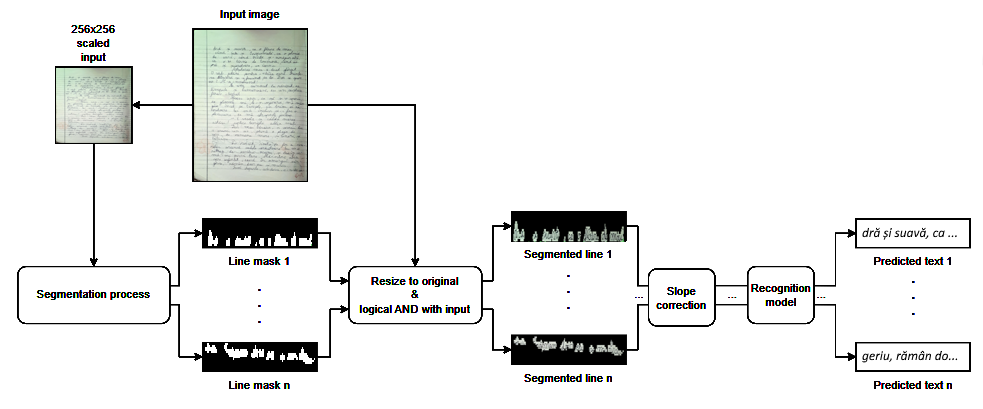
\includegraphics[scale=0.6]{figures/workflow_diagram.png}
    \caption{Schematic description of the method}
    \label{FigWorkflow}        
\end{figure}

The solution (briefly illustrated in Figure \ref{FigWorkflow}) consists of two main steps, namely the segmentation and the recognition process. For the segmentation part, the input image is scaled to a lower size in order to reduce the information load, since detecting the text layout is better facilitated by the general view rather than minor high-resolution details. A neural network model followed by some post-processing steps (which will be detailed in the next section) produces a binary mask for each line of text the segmentation detects. Each mask should highlight the portions of image that contains handwritten characters and cancel everything that is not text. Afterwards, the masks are compared against the original image and each line is obtained through a pixelwise AND operation. Finally, a recognition model computes a textual prediction for each of those segmented lines. The results can be either presented as-is, or concatenated into a single output representing the text read from the entire image.
